%
\documentclass[12pt]{article}

% The usual packages
\usepackage{fullpage}
\usepackage{breakcites}
\usepackage{setspace}
\usepackage{endnotes}
%\usepackage{float} % can't use with floatrow
\usepackage{amsmath}
\usepackage{amsfonts}
\usepackage{amssymb}
\usepackage{rotating}
\usepackage{longtable}
\usepackage{microtype}
\usepackage{graphicx}
\usepackage{hyperref}
%\usepackage[usenames,dvipsnames]{color}
\usepackage{url}
\usepackage{natbib}
\usepackage{framed} 
\usepackage{epigraph}
\usepackage{lipsum}
\usepackage{enumerate}
%\usepackage{dcolumn}
%\restylefloat{table}
\bibpunct{(}{)}{;}{a}{}{,}

% Set paragraph spacing the way I like
\parskip=0pt
\parindent=20pt

%\usepackage{helvet}
\usepackage[labelfont={bf}, margin=0cm, font=small, skip=0pt]{caption}


% Define mathematical results
\newtheorem{lemma}{Lemma}
\newtheorem{proposition}{Proposition}
\newtheorem{theorem}{Theorem}
\newtheorem{claim}{Claim}
\newenvironment{proof}[1][Proof]{\begin{trivlist}
\item[\hskip \labelsep {\bfseries #1}]}{\end{trivlist}}
\newenvironment{definition}[1][Definition]{\begin{trivlist}
\item[\hskip \labelsep {\bfseries #1}]}{\end{trivlist}}
\newenvironment{example}[1][Example]{\begin{trivlist}
\item[\hskip \labelsep {\bfseries #1}]}{\end{trivlist}}
\newenvironment{remark}[1][Remark]{\begin{trivlist}
\item[\hskip \labelsep {\bfseries #1}]}{\end{trivlist}}
\DeclareMathOperator*{\argmin}{arg\,min}
\DeclareMathOperator{\med}{med}


% Set up fonts the way I like
%\usepackage{tgpagella}
%\usepackage[T1]{fontenc}
%\usepackage[bitstream-charter]{mathdesign}

%% Baskervald
%\usepackage[lf]{Baskervaldx} % lining figures
%\usepackage[bigdelims,vvarbb]{newtxmath} % math italic letters from Nimbus Roman
%\usepackage[cal=boondoxo]{mathalfa} % mathcal from STIX, unslanted a bit
%\renewcommand*\oldstylenums[1]{\textosf{#1}}

%\usepackage[T1]{fontenc}
%\usepackage{newtxtext,newtxmath}

% A special command to create line break in table cells
\newcommand{\specialcell}[2][c]{%
 \begin{tabular}[#1]{@{}c@{}}#2\end{tabular}}


%% Set up lists the way I like
% Redefine the first level
\renewcommand{\theenumi}{\arabic{enumi}.}
\renewcommand{\labelenumi}{\theenumi}
% Redefine the second level
\renewcommand{\theenumii}{\alph{enumii}.}
\renewcommand{\labelenumii}{\theenumii}
% Redefine the third level
\renewcommand{\theenumiii}{\roman{enumiii}.}
\renewcommand{\labelenumiii}{\theenumiii}
% Redefine the fourth level
\renewcommand{\theenumiv}{\Alph{enumiv}.}
\renewcommand{\labelenumiv}{\theenumiv}
% Eliminate spacing around lists
\usepackage{enumitem}
\setlist{nolistsep}

% Create footnote command so that my name
% has an asterisk rather than a one.
\long\def\symbolfootnote[#1]#2{\begingroup%
\def\thefootnote{\fnsymbol{footnote}}\footnote[#1]{#2}\endgroup}

% Create the colors I want
\usepackage{color}
\definecolor{darkred}{RGB}{100,0,0}

\hypersetup{
pdftitle={When BLUE Is Not Best}, % title
pdfauthor={Dan K. Baissa and Carlisle Rainey}, % author
pdfkeywords={robust linear regression} {outliers} {leverage}
pdfnewwindow=true, % links in new window
colorlinks=true, % false: boxed links; true: colored links
linkcolor=black, % color of internal links
citecolor=black, % color of links to bibliography
filecolor=black, % color of file links
urlcolor=blue % color of external links
}

% section headers
%\usepackage[scaled]{helvet}
%\renewcommand\familydefault{\sfdefault} 
%\usepackage[T1]{fontenc}
%\usepackage{titlesec}
%\titleformat{\section}
%  {\normalfont\sffamily\Large\bfseries}
%  {\thesection}{1em}{}
%\titleformat{\subsection}
%  {\normalfont\sffamily\large\bfseries}
%  {\thesection}{1em}{}
%  \titleformat{\subsubsection}
%  {\normalfont\sffamily\bfseries}
%  {\thesection}{1em}{}

% enable comments in pdf
\newcommand{\dtk}[1]{\textcolor{blue}{#1}}
\newcommand{\ctk}[1]{\textcolor{red}{#1}}


\begin{document}

\begin{center}
{\LARGE \textbf{Appendix for ``When BLUE Is Not Best''}\symbolfootnote[1]{We thank Bill Clark and Matt Golder for making their data available to us. The analyses presented here were conducted with \texttt{R} 3.2.2. All data and computer code necessary for replication are available at \href{https://github.com/carlislerainey/heavy-tails}{
github.com/carlislerainey/heavy-tails}.}}\\\vspace{2mm}


\vspace{10mm}

Daniel K. Baissa\symbolfootnote[2]{Daniel K. Baissa is a Ph.D. student in the Department of Government, Harvard University, 1737 Cambridge St., Cambridge, MA, 02138 (\href{mailto:dbaissa@g.harvard.edu}{dbaissa@g.harvard.edu}).}

\vspace{3mm}

Carlisle Rainey\symbolfootnote[3]{Carlisle Rainey is Associate Professor of Political Science, Florida State University, Room 531B Bellamy Building, 113 Collegiate Loop, Tallahassee, FL, 32306 (\href{mailto:crainey@fsu.edu}{crainey@fsu.edu}).}
\end{center}

\onehalfspace

\section*{Replication of Clark and Golder (2006)}

\cite{ClarkGolder2006} attempt to ``rehabilitate'' Duverger's (\citeyear{Duverger1963}) classic explanation for the number of political parties in a system.
They write: 

\begin{quote}
According to Duverger, the mechanical effect of electoral institutions favoring large parties creates incentives for strategic entry and strategic voting. 
Parties without a chance of winning are encouraged to withdraw. 
If these parties fail to withdraw, then voters will have an incentive to vote strategically in favor of better placed parties. 
Thus disproportional systems with low district magnitudes are likely to reduce the demand for political parties created by social heterogeneity (p. 694).
\end{quote}

For our replication, we focus specifically on their hypothesis:
\begin{quote}
\textsc{Hypothesis:} Social heterogeneity increases the number of electoral parties only when the district magnitude is sufficiently large.
\end{quote}

This suggests that the marginal effect of social heterogeneity should be positive and statistically significant under permissive electoral rules (i.e., large district magnitude) and about zero and statistically insignificant (though see Rainey 2014) under restrictive electoral rules (i.e., district magnitude near one).

To measure their key outcome variable, the number of political parties, Clark and Golder use the \textit{effective} number of political parties (ENEP), where $\text{ENEP} = \sum_{i = 1}^n\frac{1}{v_i^2}$, for $v_i$ represents the vote share of party $i$ in the election. 
Similarly, for their measure of social heterogeneity, Clark and Golder use the effective number of ethnic groups (ENEG), taken from Fearon's (2003) measure of ethnic fragmentation. 
To measure the restrictiveness of the electoral rules, Clark and Golder use the average district magnitude in the election. 

Figure~\ref{fig:cg-scatter} plots the key explanatory variables, district magnitude and the effective number of ethnic groups, along the horizontal and vertical axes, respectively. 
The size of the points indicates the effective number of political parties for each election. 
The hypothesis predicts that the large points should lie in the upper-right section of the plot and small points should lie near the horizontal and vertical axes.

\begin{figure}[h!]
\begin{center}
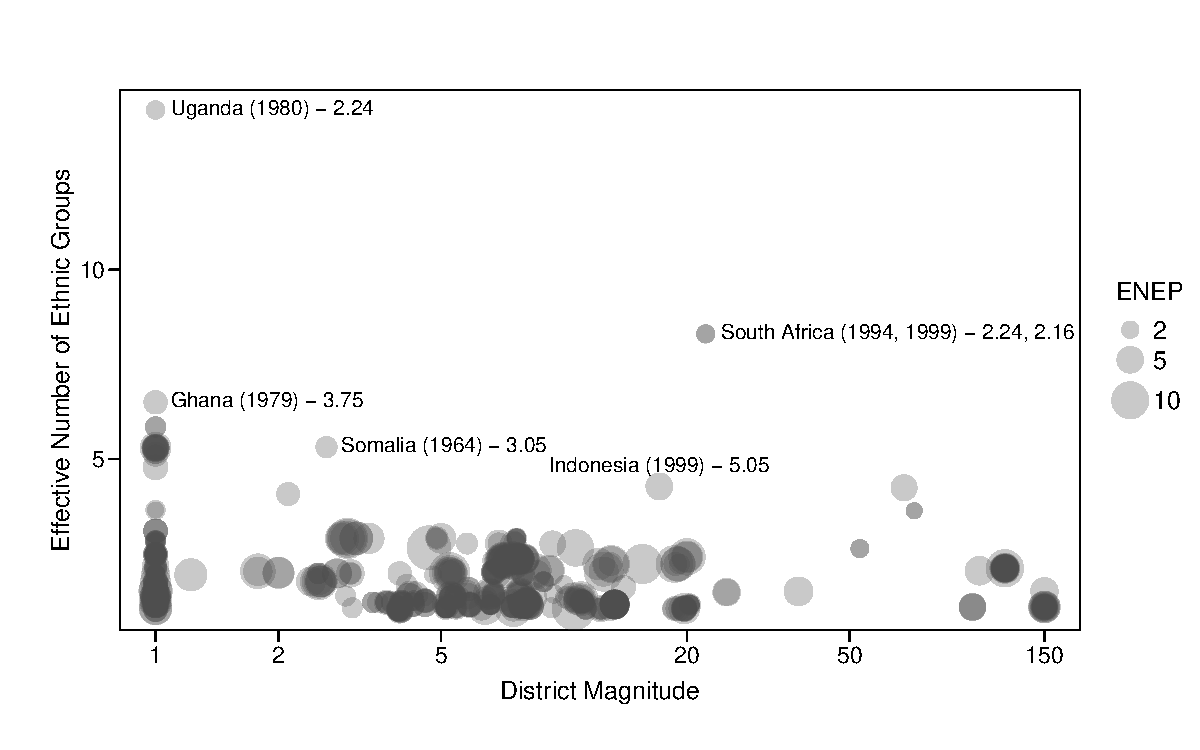
\includegraphics[scale = 0.8]{figs/cg-scatter.pdf}
\caption{The distribution of district magnitude (on the log scale) and ethnic heterogeneity.\\
Note: the point sizes indicate the number of political parties. 
According to Clark and Golder's hypothesis, large points should lie in the upper-right portion of the plot and small points should lie along the axes.}\label{fig:cg-scatter}
\end{center}
\end{figure}

To test this hypothesis, Clark and Golder fit the following linear model using least squares:
\begin{align}
\begin{split}
\text{ENEP}_i = \beta_0 &+ \beta_1 \text{ENEG}_i + \beta_2 \log(\text{Magnitude}_i) + \beta_3 \text{Upper-Tier Seats}_i\\
                                                     &+\beta_4 \text{Presidential Candidates}_i + \beta_5 \text{Proximity}_i\\
                                                     &+ \beta_6 \text{Ethnic}_i \times \log (\text{Magnitude}_i) + \beta_7 \text{Ethnic}_i \times \text{Upper-Tier Seats}_i\\
                                                     &+ \beta_8 \text{Presidential Candidates}_i \times \text{Proximity}_i + \epsilon_i\text{ ,}
\end{split}                                                     
\end{align}

The first key coefficient in this analysis is $\beta_1$, which captures the effect of social heterogeneity when district magnitude is one (i.e., the log of district magnitude is zero) and there are no upper-tier seats. 
According to the hypothesis, $\beta_1$ should be about zero. 
The second key coefficient is $\beta_6$, which captures how the effect of social heterogeneity changes with the electoral rules. 
According to the hypothesis, $\beta_6$ should be positive, so that the effect of social heterogeneity becomes (perhaps more) positive as the district magnitude increases.

Clark and Golder use least squares to obtain their estimates of the model coefficients, but worry about their estimates of the standard errors. 
They write that ``[t]he crucial thing to remember is that although OLS is consistent with longitudinal data, the standard errors may be incorrect'' (p. 690). 
They discuss several options and ultimately settle on robust standard errors clustered by country, but show that their conclusions are robust to alternative approaches to estimating standard errors. 
However, they do not address the possibility of a non-normal error distribution or its potential impact on the coefficient estimates. 
This is especially concerning given that the effective number of electoral parties is bounded below by zero, perhaps creating an error distribution with a skew to the right. 

To get an initial sense of how the results might change using an alternative (perhaps more efficient) estimator, we replicated the estimates from four models in their Table 2 using least squares and the biweight estimator. 
For these initial estimates, we make no attempt to account for the clustered nature of the data in calculating the standard errors, but do supply the usual 90\% confidence intervals to serve as a lower-bound on the uncertainty. 
Figure~\ref{fig:cg-coef-plots} presents these estimates and confidence intervals.

\begin{figure}[h!]
\begin{center}
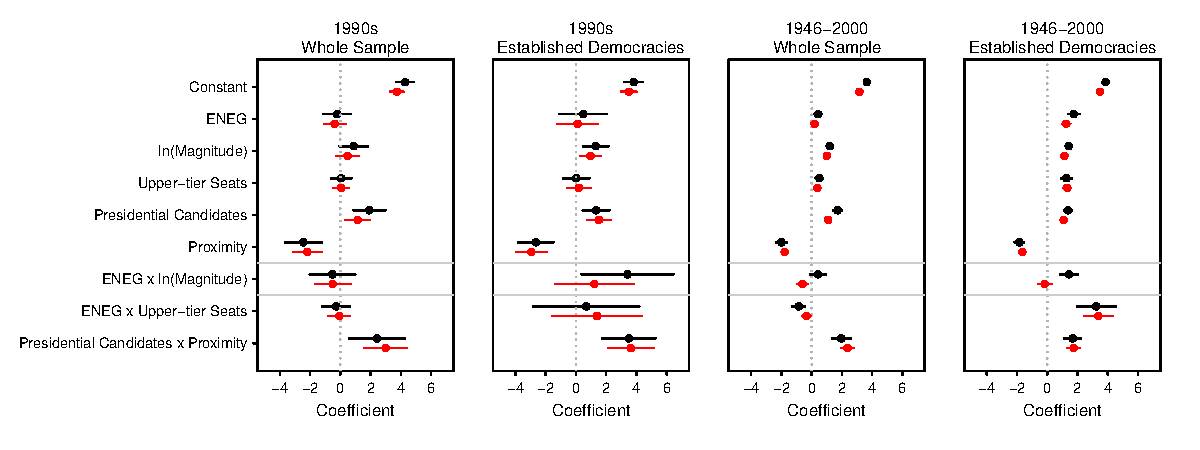
\includegraphics[scale = .8]{figs/cg-coef-plots.pdf}
\caption{Coefficient estimates of Clark and Golder's (2006) linear model using a least-squares and biweight estimator.\\
Note: the explanatory variables are standardized to have mean zero and standard deviation one-half. 
The black lines and points show the least squares estimates and 90\% confidence intervals and the red lines and points show the biweight estimates and confidence intervals. 
Notice that the coefficient for the product of the effective number of ethnic groups and the district magnitude changes drastically with the choice of estimator.}\label{fig:cg-coef-plots}
\end{center}
\end{figure}

The crucial estimate $\hat{\beta}_6$ changes substantially depending on the choice of estimator. 
This key estimate, which the theory suggests should be positive, remains negative in the 1990s sample including new democracies, shrinks substantially toward zero in the 1990s sample that includes only established democracies, and \textit{becomes negative} in the large sample of countries from 1946--2000 that includes new democracies \textit{and} the large sample that only includes established democracies. 
When results depend on the choice of estimator, it is especially important to carefully examine the residuals.

For the remainder of our analysis, we focus on the estimates from large sample of countries from 1946--2000 that includes only established democracies. 
Figure~\ref{fig:cg-residuals-hist} presents the histogram of the residuals from the least-squares estimates and Figure~\ref{fig:cg-qq-plot} presents the QQ plot for these residuals. 
Both figures indicate a substantial skew to the right. 
While this does not necessarily lead to biased estimates, it does, in our view, suggest that the linear model would be more appropriate for a transformed outcome variable. 
If the transformation makes the errors more closely approximate a normal distribution, then the least squares estimators will be more efficient. 
The model for the transformed outcome can capture potentially interesting substantive effects as well.

\begin{figure}[h!]
\begin{center}
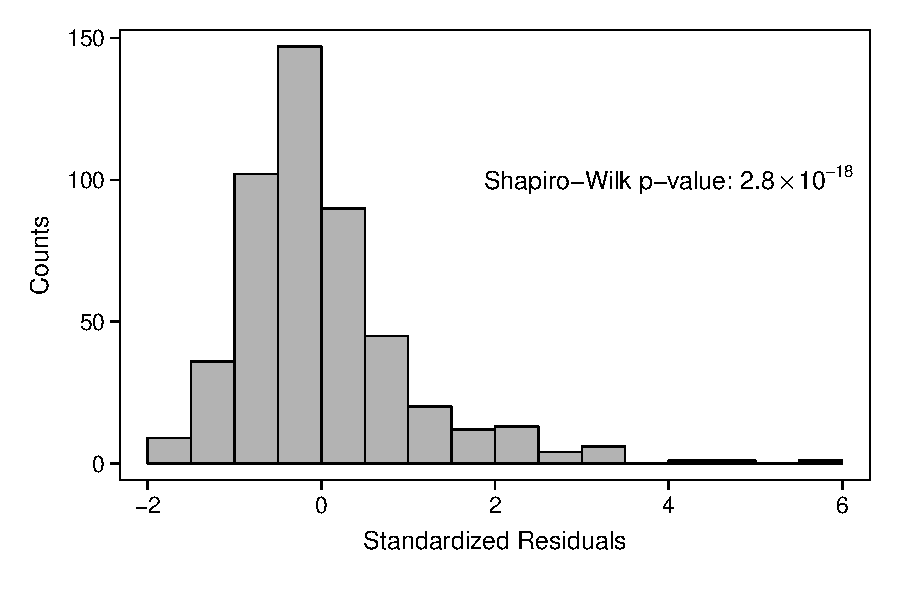
\includegraphics[scale = 0.6]{figs/cg-residuals-hist.pdf}
\caption{A histogram of the residuals from Clark and Golder's (2006) main model.\\
Note: the residuals are not approximately normal, but have a strong skew to the right. 
For example, one would rarely expect to observe residuals more that three standard deviations from zero if the assumption of normality holds. 
In these data, we have several residuals more that three standard deviations away and one nearly six standard deviations away, suggesting that some transformation of the outcome variable might be useful.}\label{fig:cg-residuals-hist}	
\end{center}
\end{figure}

\begin{figure}[h!]
\begin{center}
	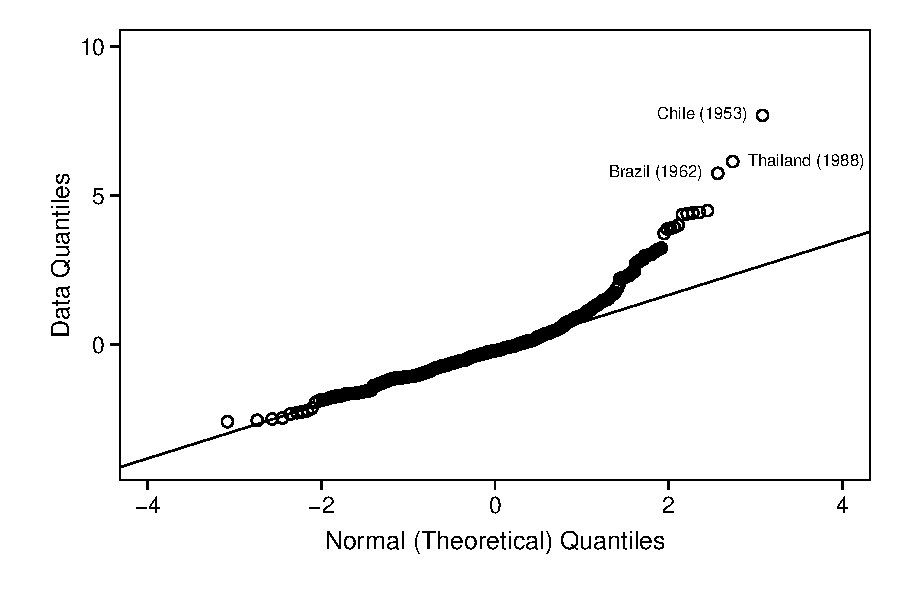
\includegraphics[scale = 0.6]{figs/cg-qq-plot.pdf}
\caption{QQ plot of the residuals in Clark and Golder's (2006) main model.\\
Note: if the residuals were approximately normal, then the points in the QQ plot would approximately follow the plotted line. 
However, notice that the positive residuals deviate sharply from the theoretical expectations. 
This also suggests that some transformation of the outcome variable might be useful.}\label{fig:cg-qq-plot}
\end{center}

\end{figure}

The maximum likelihood estimate of the Box-Cox transformation parameter $\lambda$ is about $-\frac{1}{3}$ and the confidence interval does not include zero, which suggests that a log-transformation does not quite eliminate the skew. 
We re-estimated the model using both a log-transformation and Box-Cox transformation with $\lambda = -\frac{1}{3}$. 
Figure~\ref{fig:cg-trans-residuals-hist} presents the histograms of the residuals from these two regression models. 
Notice that log-transforming the effective number of electoral parties does not quite eliminate the skew in the residuals. However, the Box-Cox transformation with $\lambda = -\frac{1}{3}$ produces highly symmetric residuals. 

\begin{figure}[h!]
\begin{center}
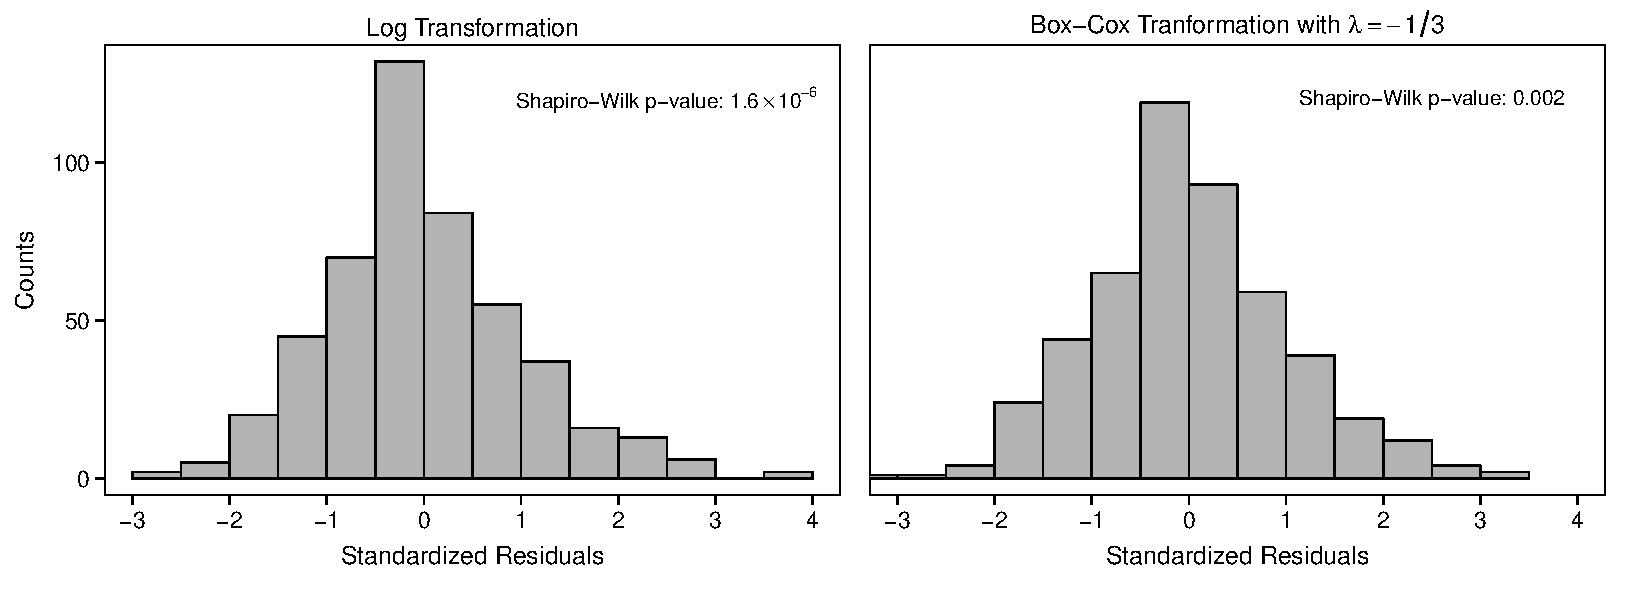
\includegraphics[width = \textwidth]{figs/cg-trans-residuals-hist.pdf}
\caption{Histograms of the residuals after transforming the outcome variable. \\
Note: the left panel shows that the log transformation does not quite remove all of the skew, but the right panel shows that the Box-Cox transformation with $\lambda = -\frac{1}{3}$ creates an approximately symmetric error distribution.}\label{fig:cg-trans-residuals-hist}
\end{center}
\end{figure}

Figure~\ref{fig:cg-trans-qq-plot} shows the QQ plot for the residuals. 
The left panel confirms that a right-skew remains after the log-transformation, as suggested by the histogram in the left panel of Figure~\ref{fig:cg-trans-residuals-hist}. 
The right panel of Figure~\ref{fig:cg-trans-qq-plot} confirms that the Box-Cox transformation removes much or all of this skew, as suggested by the right panel of Figure~\ref{fig:cg-trans-residuals-hist}. 

\begin{figure}[h!]
\begin{center}
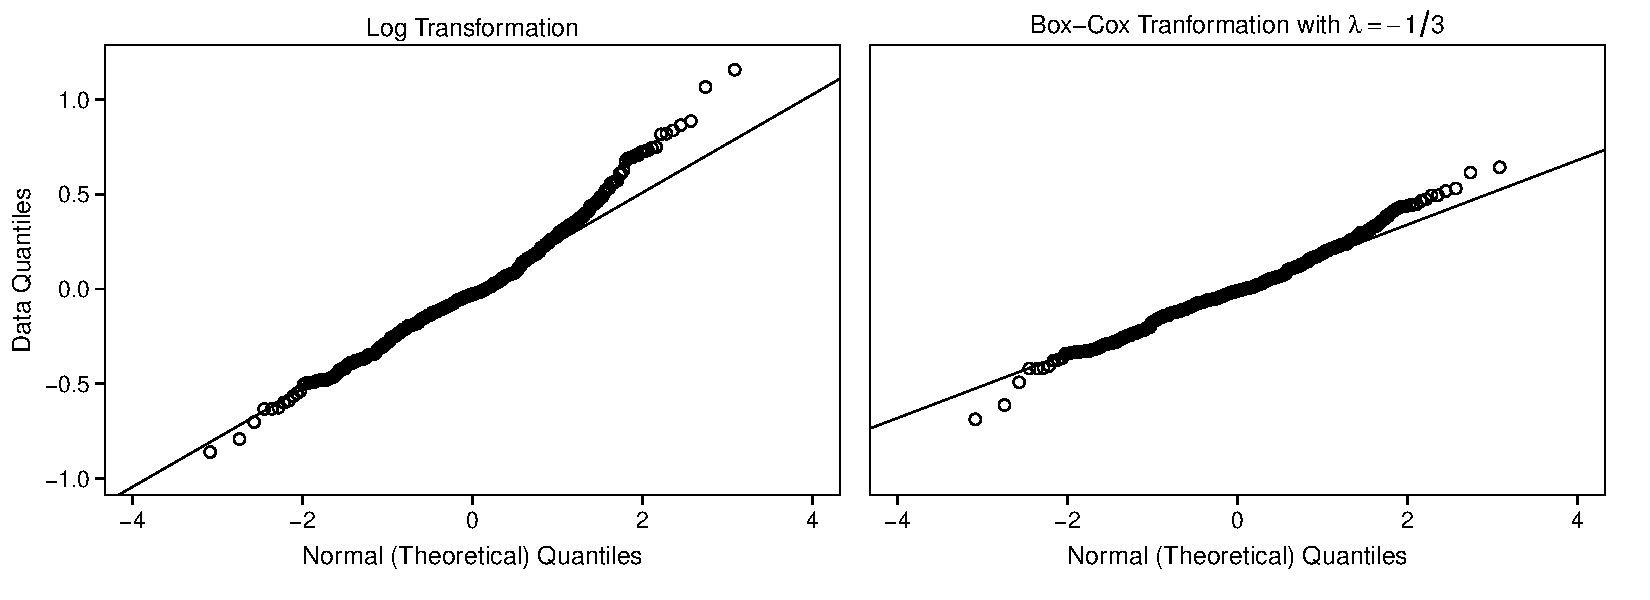
\includegraphics[width = \textwidth]{figs/cg-trans-qq-plot.pdf}
\caption{QQ plots of the residuals after transforming the outcome variable.\\
Note: the left panel shows that the log transformation does not quite remove all of the skew, but the right panel shows that the Box-Cox transformation with $\lambda = -\frac{1}{3}$ creates an approximately symmetric error distribution, though it has heavier tails than a normal distribution.}\label{fig:cg-trans-qq-plot}
\end{center}
\end{figure}

Although the Box-Cox transformation removes much or all of the skew, the residuals retain tails that are slightly heavier than the tails of the normal distribution. 
The residuals have larger positive and negative quantiles than one would expect under a normal distribution. 
This suggests the residuals follow a heavy-tailed distribution, perhaps resembling a $t$ distribution with degrees of freedom in the range of six to twelve. 
Even after the Box-Cox transformation, the Shapiro-Wilk test rejects the null hypothesis of normality with $p = 0.002$. 
Assuming that these residuals follow a $t$-distribution, we can estimate the degrees of freedom using maximum likelihood, which points toward a $t$ distribution with about ten degrees of freedom. 
Recall that the biweight estimator is a (slightly) more efficient estimator for $t_{10}$ distributed errors. 
However, because the least squares estimator eliminates large errors at the expense of many small and moderate errors, the error distribution might have \textit{even heavier} tails than the least squares estimates suggest.

Most importantly, after the Box-Cox transformation, the residuals are well-behaved. 
They are highly symmetric and only slightly heavy-tailed. 
In spite of a nearly ideal situation, the simulations in Table 1 and Figure 2 in the main text suggest that the biweight estimate is slightly more efficient in this application. 
But these differences are slight so it can be valuable to carefully examine a least squares estimator and a more robust estimator.

\subsection*{Quantities of Interest}

To estimate the quantity of interest---the effect of social heterogeneity as the permissiveness of the electoral rules varies---we re-estimate Clark and Golder's model with and without the Box-Cox transformation using both the least squares and biweight estimators. 
To obtain standard errors, we use the cluster bootstrap suggested by \cite{Harden2012} to calculate the confidence intervals for each model.

Figure~\ref{fig:cg-fd-plots} shows the effect of increasing social heterogeneity from ENEG = 1.06 (10th percentile) to ENEG = 2.48 (90th percentile) as the district magnitude varies. 
The upper-left figure replicates Clark and Golder's approach (except for the cluster-bootstrap confidence intervals) and replicates their finding, which they summarize:

\begin{quote}
[These results] clearly illustrate that in established democracies, ethnic heterogeneity significantly increases the number of parties once the electoral system is sufficiently permissive. 
This is exactly what Duverger's theory predicts. 
To be more specific, Figure 1a [our upper-left panel of Figure~\ref{fig:cg-fd-plots}], based on the pooled model with established democracies, indicates that ethnic heterogeneity will increase the number of electoral parties once we move beyond nonpermissive electoral systems with single-member districts when [Magnitude = 1].
\end{quote}

\begin{figure}[h!]
\begin{center}
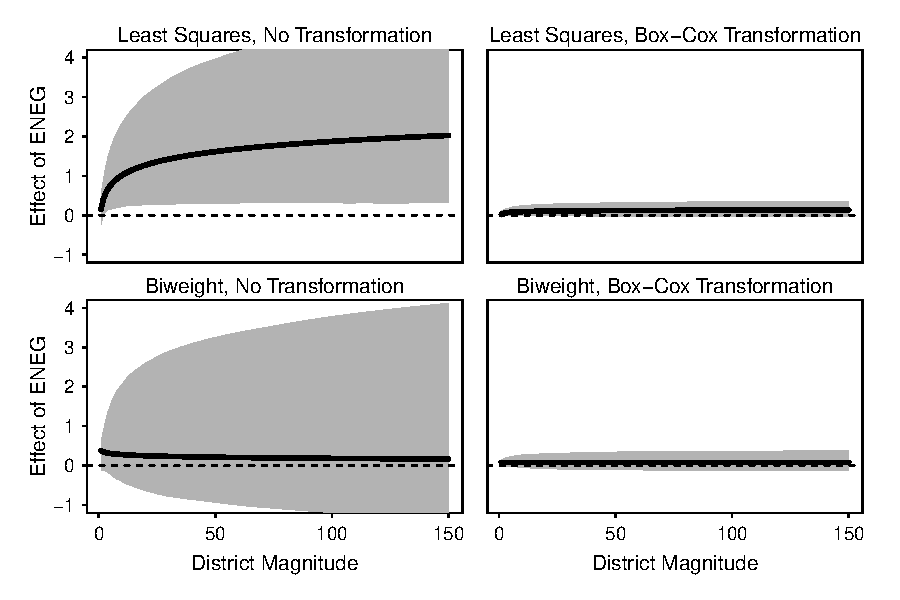
\includegraphics[width = \textwidth]{figs/cg-fd-plots.pdf}
\caption{The estimated effects and 90\% confidence intervals of increasing social heterogeneity from ENEP = 1.06 (10th percentile) to ENEP = 2.48 (90th percentile) on the effective number of electoral parties as the district magnitude varies. \\
Note: only the model that does not use robust estimators or transform the outcome variable provides evidence in support of the hypothesis.}\label{fig:cg-fd-plots}
\end{center}
\end{figure}

But this evidence breaks down once we adjust for the non-normality of the errors. 
The lower-left panel of Figure~\ref{fig:cg-fd-plots} shows that using the biweight estimator as a robust alternative to least squares produces estimated interaction in the \text{opposite} direction as the hypothesis predicts, though small and not statistically significant. 
The upper-right panel of Figure~\ref{fig:cg-fd-plots} shows that transforming the outcome variable to make the data more consistent with the assumed normal-linear model substantially increases the uncertainty across the range of district magnitude, so that small negative effects are now plausible, as well as much larger positive effects. 

However, we argue that the best approach for these data is to transform the outcome variable to obtain a roughly symmetric error distribution \textit{and} use the biweight estimator to address the remaining heavy tails shown in the left panel of Figure~\ref{fig:cg-trans-qq-plot}. 
This approach reduces effect of social heterogeneity somewhat across the range of district magnitude.

Because the scale of the estimates and uncertain differ drastically across the choice to transform the outcome variable or not, as well as the range of district magnitude, we present the relevant quantities of interest in Table~\ref{tab:cg-qi}. 
In this case, we are interested in the effect of substantially increasing social heterogeneity from ENEG = 1.06 (10th percentile) to ENEG = 2.48 (90th percentile) on the number of political parties when district magnitude is one (10th percentile) and also when district magnitude is 14 (90th percentile). 
Since the hypothesis suggests that this effect should be larger when the district magnitude is larger, we are also interested in the difference between these two effects. 
For simplicity, we focus our discussion on the differences between the typical approach, least squares with no transformation, and the approach we recommend, transformation \textit{and} robust estimation.

The first row of Table~\ref{tab:cg-qi} suggests that in countries with single-member districts, a substantial increase in ENEG (10th to 90th percentile) increases the ENEP by about 0.16 [-0.24; 0.53] parties. 
On the other hand, in large, multimember districts (magnitude of 14), the same increase in social heterogeneity increases the ENEP by about 1.14 [0.26; 2.67] parties. 
This is just as the hypothesis predicts. 
Further, this increase of 0.98 [0.06; 2.65] is large and statistically significant.\footnote{Using cluster-robust standard errors, Clark and Golder find that the product term is \textit{not quite} significant. We use cluster-bootstrap standard errors and find the coefficient is \textit{barely} significant.}

\begin{table}[h!]
{\scriptsize
% quantreg::latex.table(x = qitab, file = "doc/tabs/cg-qi", rowlabel = "",      rowlabel.just = "l", cgroup = c("First-Difference When \\textit{M} = 1",          "First-Difference When \\textit{M} = 14", "Second-Difference"),      rgroup = c("No Transformation", "Box-Cox Transformation"),      n.rgroup = c(2, 2), table.env = FALSE) 
%
\begin{center}
\begin{tabular}{|l||c|c||c|c||c|c|} \hline
\multicolumn{1}{|l||}{\bf }&\multicolumn{2}{c||}{\bf First-Difference When \textit{M} = 1}&\multicolumn{2}{c||}{\bf First-Difference When \textit{M} = 14}&\multicolumn{2}{c|}{\bf Second-Difference}\\ \cline{2-7}
\multicolumn{1}{|l||}{}&\multicolumn{1}{c|}{Est.}&\multicolumn{1}{c||}{90\% CI}&\multicolumn{1}{c|}{Est.}&\multicolumn{1}{c||}{90\% CI}&\multicolumn{1}{c|}{Est.}&\multicolumn{1}{c|}{90\% CI}\\ \hline
{\bf No Transformation}&&&&&&\\
~~Least Squares&~~~~~0.16~~~~~&[-0.24;~~0.53]&~~~~~1.14~~~~~&[0.26;~2.67]~~&~~~~~0.98~~~~~&[0.06;~2.65]~~\\ 
~~Biweight&~~~~~0.37~~~~~&[-0.12;~~0.62]&~~~~~0.26~~~~~&[-0.51;~~2.33]&~~~~~-0.11~~~~&[-0.96;~~2.05]\\ \hline
{\bf Box-Cox Transformation}&&&&&&\\
~~Least Squares&~~~~~0.03~~~~~&[-0.05;~~0.12]&~~~~~0.10~~~~~&[0.00;~0.26]~~&~~~~~0.07~~~~~&[-0.07;~~0.26]\\ 
~~Biweight&~~~~~0.08~~~~~&[-0.04;~~0.15]&~~~~~0.08~~~~~&[-0.06;~~0.28]&~~~~~0.00~~~~~&[-0.17;~~0.25]\\ 
\hline
\end{tabular}
\end{center}

}
\caption{The quantities of interest from least squares and biweight estimates, with and without the Box-Cox transformation of the outcome variable. \\
Note: the least squares estimates without transforming the outcome variable are consistent with Clark and Golder's hypothesis. 
However, transforming the outcome variable, using the robust biweight estimator,  or both substantially reduces the amount of evidence that these data offer in favor of the hypothesis.}\label{tab:cg-qi}
\end{table}

However, once we make an effort to account for the non-normality of the residuals by transforming the outcome variable \textit{and} using the robust biweight estimator, this evidence for interaction weakens slightly. 
This model suggests that, in single-member districts, a substantial increase in social heterogeneity increases the ENEP by about 0.29 [-0.13; 0.48] parties. 
This is about twice Clark and Golder's initial estimate.
In large, multimember districts (magnitude of 14), the estimate shrinks to 0.62 [-0.41; 3.34], which is about half of Clark and Golder's estimate. 
This leads to an estimated increase of 0.33 [-0.78; 3.14] in the effect of social heterogeneity as we move from single-member districts to large, multimember districts---about one-third of Clark and Golder's initial estimate.

\subsection*{Differences Between the Estimates}

One major advantage of robust estimators is that these estimators allow unusual cases to stand out. 
Figure~\ref{fig:cg-residuals-compare} compares the residuals from the least squares fit and the biweight fit after the Box-Cox transformation. 
Notice that the residuals tend to agree, except for the 1980 election in Uganda, which is the largest residual in the biweight fit, but does not stand out among the least squares residuals.

\begin{figure}[h!]
\begin{center}
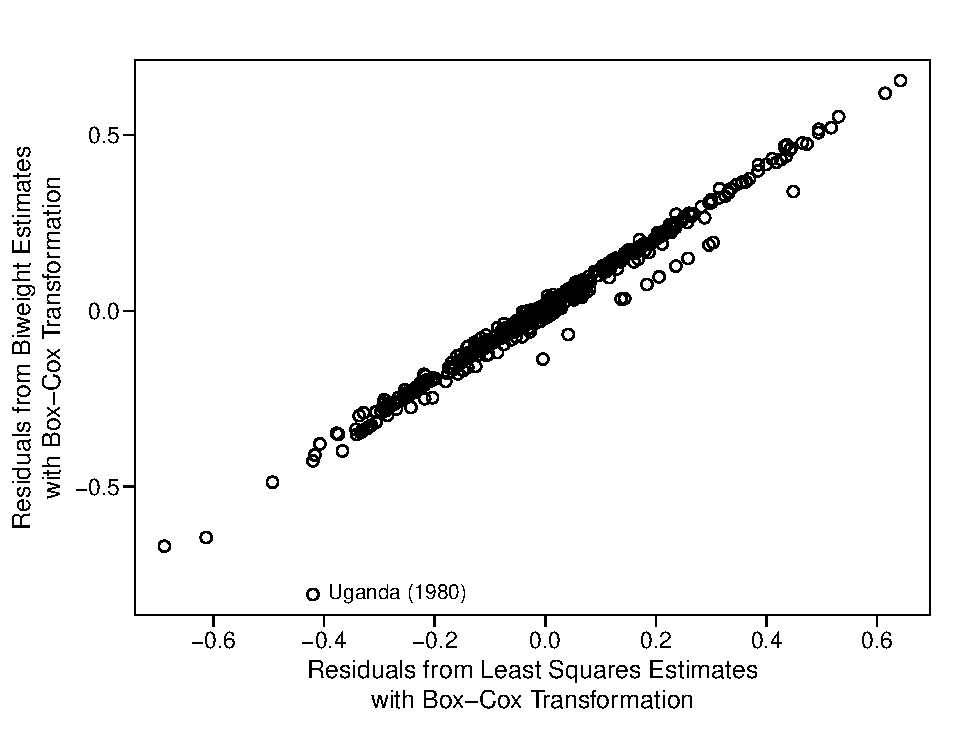
\includegraphics[scale = 0.6]{figs/cg-residuals-compare.pdf}
\caption{The relationship between the least squares and biweight estimates after the Box-Cox transformation. \\
Note: the biweight estimate allows the unusual case of Uganda to stand out from the others.}\label{fig:cg-residuals-compare}
\end{center}
\end{figure}

Similarly, Figure~\ref{fig:cg-weights} presents the 35 smallest weights from the biweight fit. 
Recall that as cases become increasingly inconsistent with most of the data, the biweight estimator increasingly downweights these cases, potentially to zero. 
As we might expect, given the residuals in Figure~\ref{fig:cg-residuals-compare}, the 1980 election in Uganda receives zero weight. 
This election is consistent with the hypothesis because it features single member districts, an extremely large number of ethnic groups, and only two major political parties. 
Unfortunately for the hypothesis, though, this case is inconsistent with most of the data.

\begin{figure}[h!]
\begin{center}
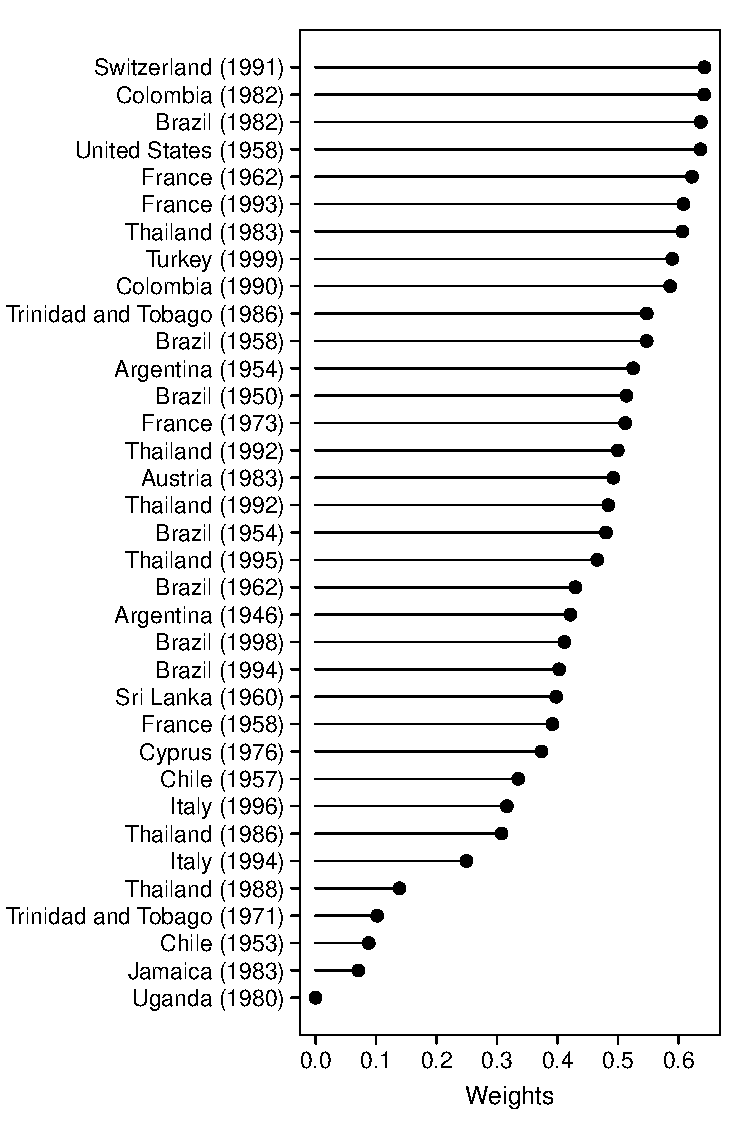
\includegraphics[scale = 0.7]{figs/cg-weights.pdf}
\caption{The final weights implied by the biweight estimator. \\
Note: because the 1980 election in Uganda is quite different from the remainder of the data, the biweight estimator downweights this case all the way to zero.}\label{fig:cg-weights}
\end{center}
\end{figure}


\singlespace
\bibliographystyle{apsr_fs}
\bibliography{bibliography.bib}

\end{document}
